\subsection*{Strømforstærker}
\label{effekt_stroemforstaerker}

\begin{figure}[h]
\centering
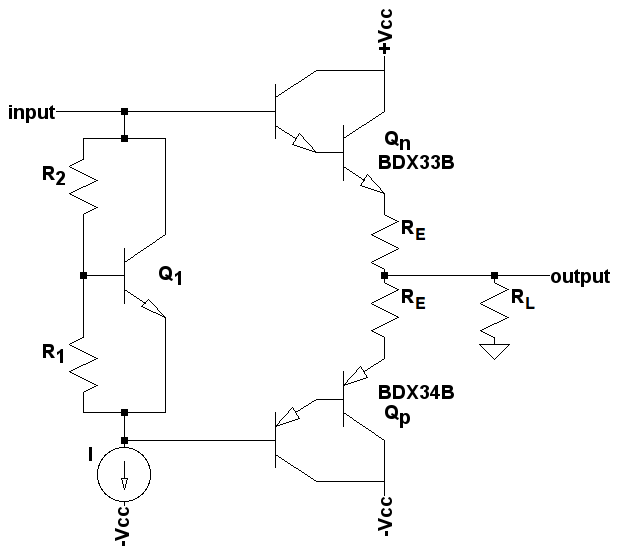
\includegraphics[scale=0.4]{teknisk/effektforstaerker/blokdiagram-stroemforstaerker.png}
\caption{Diagram over strømforstærkeren}
\label{fig:blokdiagram-stroem}
\end{figure}

Strømforstærkeren opbygges som vist på figur \ref{fig:blokdiagram-stroem}. Dog vil konstantstrømsgeneratoren blive bygget i diskret elektronik. Der er valgt at der benyttes en BDX33B og en BDX34B \fixme{kilde: BDX33-34.pdf} som udgangstransistorer. Dette er darlingtontransistorer, som er valgt da de har en $h_{\mathrm{FE}}$ på minimum 750 og kan klare en $I_C$ på op til 10 A. Desuden var de let tilgængelige til projektet.\\
Som vist, i afsnit \ref{valg_kortslutningssikring}, skal der igennem $R_{\mathrm{load}}$ løbe en $I_{\mathrm{peak}}$ på 2,24 A for at opnå en udgangseffekt på 20 W. Dette betyder desuden, som det også er vist i afsnit \ref{valg_kortslutningssikring}, at der skal være en $V_{\mathrm{peak}}$ på 17,9 V over belastningen. %Da de valgte darlingtontransistorer har en $V_{\mathrm{BE}}$ på op til 2,5 V, vælges forsyningsspændingen til $\pm$25 V, hvormed spændingsfaldet over transistorerne ikke umuliggører den tilstrækkelige spænding over belastningen. 
Modstanden $R_E$ bestemmes som det første, udfra termiske hensyn.\\\\
Størrelsen af $R_E$ tager udgangspunkt i at denne skal skabe termisk stabilitet og til bestemmelsen af denne startes der derfor med at kigge på et termisk ekvivalentdiagram for de valgte darlingtontransistorer\fixme{kilde: BDX33-34.pdf} og de tilgængelige køleplader\fixme{kilde: koeleplade.pdf}. 

\begin{figure}[h]
\centering
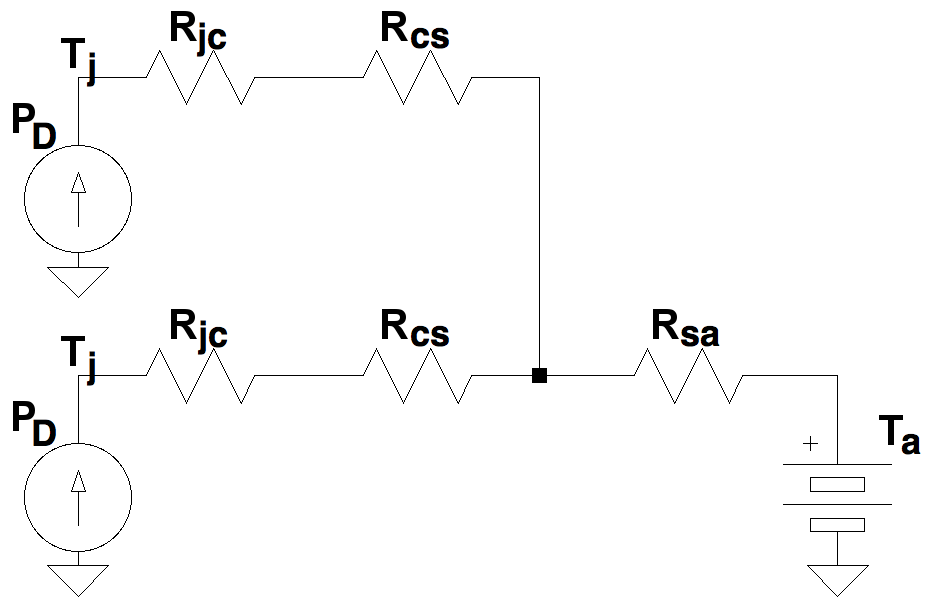
\includegraphics[scale=0.2]{teknisk/effektforstaerker/termisk_ekvivalentdiagram.png}
\caption{Termisk ekvivalentdiagram for udgangstransistorerne}
\label{fig:term-dia}
\end{figure}

På figur \ref{fig:term-dia} ses ekvivalentdiagrammet, hvor; temperatur er spænding, effekt er strøm og termisk modstand er modstand. Flere af komponenterne har samme benævnelser, da de også antager samme værdier og da der under udregningerne dermed ikke vil blive set på dem enkeltvis.\\
Størrelsen af $P_D$ er effekten afsat i en enkelt udgangstransistor og er givet ved udregningen i formel (\ref{equ:pd}). Denne formel er ganske vist gældende for klasse B udgangstrin, men i dette arbejdsområde er den også gældende for klasse AB udgangstrin\fixme{kilde: Ole}.

\begin{equation}
\label{equ:pd}
P_D = \frac{1}{\pi^2} \cdot \frac{(V_{CC})^2}{R_{\mathrm{load}}} = \frac{1}{\pi^2} \cdot \frac{(25~\mathrm{V})^2}{8~\ohm} = 7.92~\mathrm{W}
\end{equation}

Fra darlingtontransistorernes datablad haves $R_{\mathrm{jc}} = 1,78~\tfrac{\celsius}{\mathrm{W}}$ og $T_{\mathrm{j,max}} = 150~\celsius$. Databladet for kølepladen giver $R_{\mathrm{cs}} = 1,4~\tfrac{\celsius}{\mathrm{W}}$ når der anvendes isoleringspasta. Fra DIN45500 \fixme{kilde: DIN45500.pdf} fåes at HiFi-forstærkeren skal kunne holde til en omgivelsestemperatur på 35~\celsius, hvilket er $T_a$ i ekvivalentet. Udfra dette opstilles, ved simpel kredsløbsteori på ekvivalentkredsløbet på figur \ref{fig:term-dia}, formel (\ref{equ:tjmax}) til beregning af $R_{\mathrm{sa}}$ ved $T_j$  på sin maksimale værdi. 

\begin{equation}
\label{equ:tjmax}
T_j = T_a + P_D \cdot (R_{\mathrm{jc}} + R_{\mathrm{cs}} + R_{\mathrm{sa}})
\end{equation}

Desuden opstilles udfra sikkerhedshensyn\fixme{Find gerne kilde der siger dette i stedet, hvis der er tid} et krav om at kølepladen maksimalt på blive 40 \celsius, hvorved bestemmelse af $R_{\mathrm{sa}}$ også kan foregå ved brug af formel (\ref{equ:smax}). 

\begin{equation}
\label{equ:smax}
40~\celsius = 2 \cdot P_D \cdot R_{\mathrm{sa}}
\end{equation}

Det ses at formel (\ref{equ:smax}) bliver den afgørende betingelse og at $R_{\mathrm{sa}}$ maksimalt må være $2,53~\tfrac{\celsius}{\mathrm{W}}$. I databladet for kølepladen ses at en $R_{\mathrm{sa}}$ på $2,4~\tfrac{\celsius}{\mathrm{W}}$ kan opnåes ved en køleplade på 150 mm, hvilket derfor vælges. Størrelsen af $R_E$, som alt dette går ud på, kan nu bestemmes ved formel (\ref{equ:rebestem}), hvor $K = - 2~\tfrac{\mathrm{mV}}{\celsius}$, $V_{CC} = 25~V$, $V_T = 26~\mathrm{mV}$ og $I_C = 2,24~A$.

\begin{equation}
\label{equ:rebestem}
R_E = - K \cdot V_{CC} \cdot (R_{\mathrm{jc}} + R_{\mathrm{cs}} + R_{\mathrm{sa}}) - \frac{V_T}{I_C} = 535~m\ohm
\end{equation}